\documentclass[tikz,border=6pt]{standalone}

\usepackage[T1]{fontenc}
\usepackage{lmodern}
\usepackage{amsmath,amssymb}
\usepackage{xcolor}
\usetikzlibrary{shapes,arrows,positioning,calc}

\begin{document}
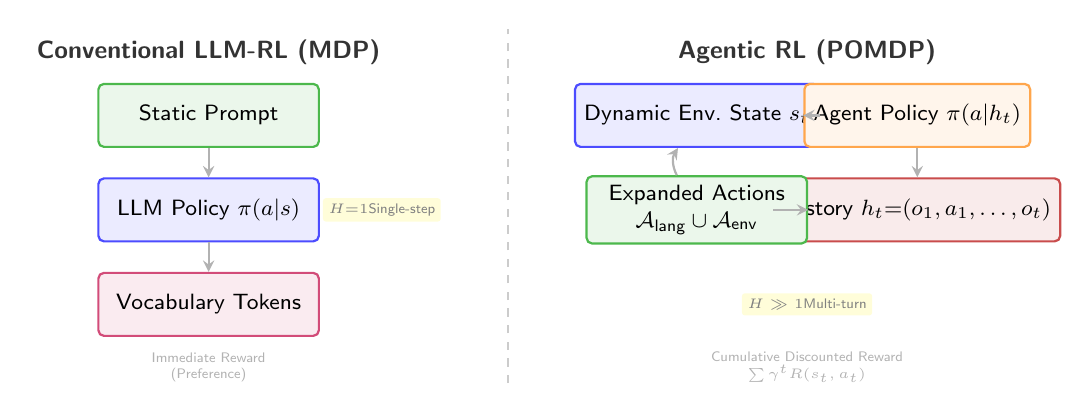
\begin{tikzpicture}[
    box/.style={rectangle, draw=#1!70, fill=#1!8, minimum width=2.8cm, minimum height=0.8cm, align=center, font=\footnotesize\sffamily, thick, rounded corners=2pt},
    arr/.style={->, >=stealth, thick, color=gray!60},
    hdr/.style={font=\small\sffamily\bfseries, text=black!80},
    note/.style={font=\tiny\sffamily, text=gray!60, align=center}
]
% --- Left panel: Conventional LLM-RL ---
\node[hdr] at (-3.8,4.2) {Conventional LLM-RL (MDP)};
\node[box=green!60!black] (sp) at (-3.8,3.4) {Static Prompt};
\node[box=blue] (llm) at (-3.8,2.2) {LLM Policy $\pi(a|s)$};
\node[box=purple] (vt) at (-3.8,1.0) {Vocabulary Tokens};
\node[note] at (-3.8,0.2) {Immediate Reward\\(Preference)};
\draw[arr] (sp) -- (llm);
\draw[arr] (llm) -- (vt);
\node[font=\tiny\sffamily, text=gray, fill=yellow!15, rounded corners=1pt, inner sep=2pt] at (-1.6,2.2) {$H{=}1$\\Single-step};

% --- Divider ---
\draw[dashed, gray!40, thick] (0,0) -- (0,4.5);

% --- Right panel: Agentic RL ---
\node[hdr] at (3.8,4.2) {Agentic RL (POMDP)};
\node[box=blue] (des) at (2.4,3.4) {Dynamic Env.\ State $s_t$};
\node[box=orange] (ap) at (5.2,3.4) {Agent Policy $\pi(a|h_t)$};
\node[box=red!70!black] (hist) at (5.2,2.2) {History $h_t{=}(o_1,a_1,\ldots,o_t)$};
\node[box=green!60!black] (ea) at (2.4,2.2) {Expanded Actions\\$\mathcal{A}_{\text{lang}} \cup \mathcal{A}_{\text{env}}$};
\node[note] at (3.8,0.2) {Cumulative Discounted Reward\\$\sum \gamma^t R(s_t,a_t)$};
\node[font=\tiny\sffamily, text=gray, fill=yellow!15, rounded corners=1pt, inner sep=2pt] at (3.8,1.0) {$H \gg 1$\\Multi-turn};
\draw[arr] (des) -- (ap);
\draw[arr] (ap) -- (hist);
\draw[arr] (hist) -- (ea);
\draw[arr, bend left=30] (ea) to (des);
\end{tikzpicture}
\end{document}